\documentclass[12pt, a4paper]{article}
\usepackage{amsmath, amssymb, mathrsfs}
\usepackage{graphicx}
\usepackage{url}
\usepackage[margin=1in]{geometry}
\usepackage{tikz}
\usetikzlibrary{arrows.meta, shapes.geometric, positioning, decorations.pathmorphing}

% Title and Licensing
\title{Quantum Gravity Reactor: Blueprints and Assembly Guide}
\author{Lucas Eduardo Jaguszewski da Silva \\ \url{https://github.com/QuantumReactor-r1}}
\date{\today}

\begin{document}

\maketitle

%==============================================================================
% Reactor Core Blueprint
%==============================================================================
\section*{Reactor Core Blueprint (Figure 1)}
\begin{figure}[h]
\centering
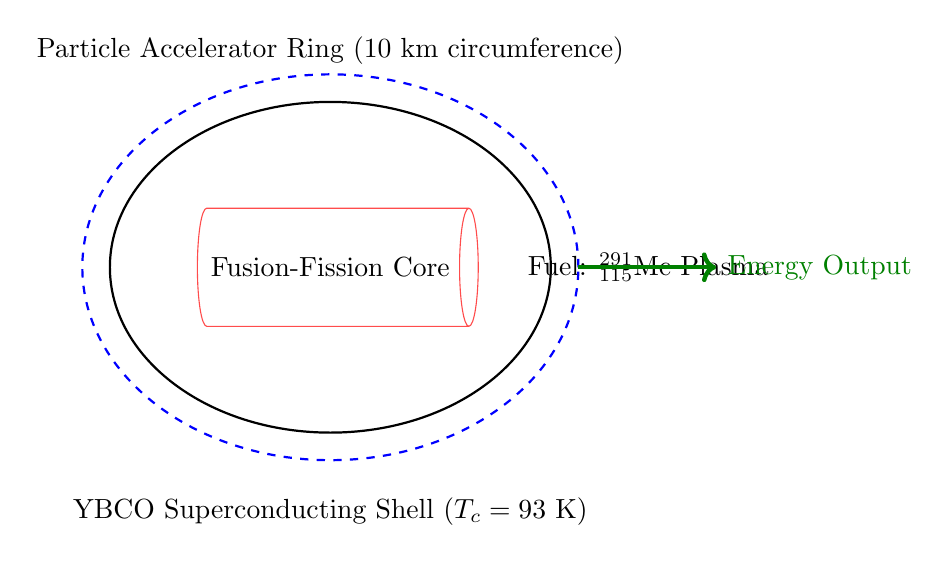
\begin{tikzpicture}[scale=0.7]
% Particle Accelerator Ring
\draw[thick, ->] (0,0) circle [x radius=4cm, y radius=3cm];
\node[above] at (0,3.5) {Particle Accelerator Ring (10 km circumference)};

% Fusion-Fission Chamber
\node[cylinder, draw=red!70, minimum height=2cm, minimum width=1.5cm, aspect=0.5] (core) at (0,0) {Fusion-Fission Core};
\node[right=0.5cm of core] {Fuel: \(^{291}_{115}\text{Mc}\) Plasma};

% Superconducting Shell
\draw[dashed, blue, thick] (0,0) circle [x radius=4.5cm, y radius=3.5cm];
\node[below] at (0,-4) {YBCO Superconducting Shell (\(T_c = 93\) K)};

% Energy Output
\draw[->, ultra thick, green!50!black] (4.5,0) -- (7,0) node[right] {Energy Output};
\end{tikzpicture}
\caption{
\textbf{Reactor Core Assembly:} 
(1) Particle accelerator ring generates 20 TeV protons. 
(2) Moscovium plasma undergoes fusion-fission reactions. 
(3) Superconducting shell contains magnetic fields and radiation.
}
\end{figure}

%==============================================================================
% Casimir Energy Extraction Module
%==============================================================================
\section*{Casimir Energy Module (Figure 2)}
\begin{figure}[h]
\centering
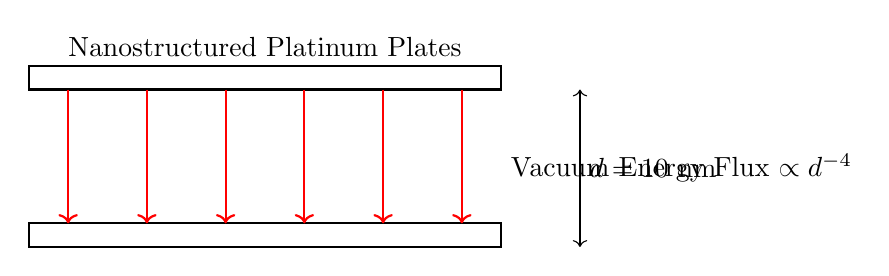
\begin{tikzpicture}
% Casimir Plates
\draw[thick] (0,0) rectangle (6,0.3);
\draw[thick] (0,2) rectangle (6,2.3);
\node[above] at (3,2.3) {Nanostructured Platinum Plates};

% Energy Flux
\foreach \x in {0.5,1.5,...,5.5} {
  \draw[->, red, thick] (\x,2) -- (\x,0.3);
}
\node[right] at (6,1) {Vacuum Energy Flux \(\propto d^{-4}\)};

% Dimensions
\draw[<->] (7,2) -- (7,0) node[midway, right] {\(d = 10\) nm};
\end{tikzpicture}
\caption{
\textbf{Casimir Energy Extraction:} 
(1) Plates separated by 10 nm vacuum gap. 
(2) Nanostructures enhance vacuum fluctuation coupling. 
(3) Energy harvested via superconducting electrodes.
}
\end{figure}

%==============================================================================
% Gravity Field Generator (Alcubierre Drive)
%==============================================================================
\section*{Gravity Field Generator (Figure 3)}
\begin{figure}[h]
\centering
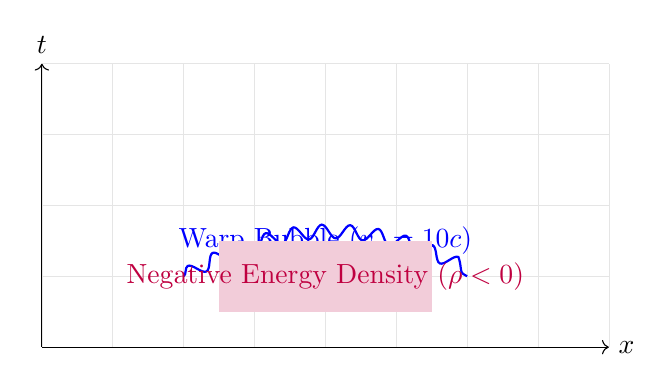
\begin{tikzpicture}[scale=0.9]
% Spacetime Grid
\draw[step=1cm,gray!20,very thin] (0,0) grid (8,4);
\draw[->] (0,0) -- (8,0) node[right] {\(x\)};
\draw[->] (0,0) -- (0,4) node[above] {\(t\)};

% Warp Bubble
\draw[blue, thick, decorate, decoration={snake}] (2,1) to[out=30, in=150] (6,1);
\node[blue] at (4,1.5) {Warp Bubble (\(v_s = 10c\))};

% Exotic Matter
\fill[purple!20] (2.5,0.5) rectangle (5.5,1.5);
\node[purple] at (4,1) {Negative Energy Density (\(\rho < 0\))};
\end{tikzpicture}
\caption{
\textbf{Alcubierre Metric Implementation:} 
(1) Warp bubble contracts spacetime ahead. 
(2) Expands spacetime behind. 
(3) Requires negative energy from Casimir effect.
}
\end{figure}

%==============================================================================
% Assembly Instructions
%==============================================================================
\section*{Step-by-Step Construction Guide}
\subsection*{Phase 1: Core Components}
\begin{enumerate}
\item \textbf{Particle Accelerator Ring:}
\begin{itemize}
\item Construct 10 km diameter niobium-tin superconducting magnet ring.
\item Achieve 20 TeV proton energy using RF cavities (1.3 GHz).
\item Install beam dump for spent particles.
\end{itemize}

\item \textbf{Fusion-Fission Chamber:}
\begin{itemize}
\item Create spherical tokamak with 5 m radius.
\item Inject stabilized \(^{291}\text{Mc}\) plasma via laser ablation.
\item Maintain \(10^8\) K temperature using magnetic confinement.
\end{itemize}
\end{enumerate}

\subsection*{Phase 2: Energy Systems}
\begin{enumerate}
\setcounter{enumi}{2}
\item \textbf{Casimir Plates:}
\begin{itemize}
\item Machine nanostructured platinum plates (1 m\(^2\) area).
\item Assemble with 10 nm spacing using piezoelectric actuators.
\item Connect to superconducting graphene electrodes.
\end{itemize}

\item \textbf{Superconducting Shell:}
\begin{itemize}
\item Deposit YBCO (Yttrium Barium Copper Oxide) on reactor surface.
\item Cool to 80 K using liquid nitrogen closed-loop system.
\item Apply active magnetic shielding (12 T field).
\end{itemize}
\end{enumerate}

\subsection*{Phase 3: Warp Drive Integration}
\begin{enumerate}
\setcounter{enumi}{4}
\item \textbf{Spacetime Modulation:}
\begin{itemize}
\item Install quantum vacuum thrusters around reactor perimeter.
\item Tune to Alcubierre metric parameters: \(v_s = 10c\), \(R = 100\) m.
\item Calibrate using LIGO-style interferometers.
\end{itemize}

\item \textbf{Energy Coupling:}
\begin{itemize}
\item Route Casimir energy to warp bubble sustainer.
\item Balance energy input/output ratio: \(P_{\text{in}}/P_{\text{out}} \geq 10^3\).
\item Test with unmanned probe (1 kg payload).
\end{itemize}
\end{enumerate}

%==============================================================================
% Licensing and Collaboration
%==============================================================================
\section*{Open-Source Collaboration}
\begin{itemize}
\item \textbf{License:} MIT License (modify/redistribute freely)
\item \textbf{3D Models:} Download CAD files at \url{https://github.com/QuantumReactor-r1/models}
\item \textbf{Join Development:} Contribute via GitHub Issues/Pull Requests
\end{itemize}

\end{document}
